\documentclass[mythesis.tex]{subfiles}
\begin{document}
% tells latex when compiling a subfile what chapter number this document is
% set the chapter to minus one as \chapter will increment the counter
\setcounter{chapter}{2} 
\chapter{Electromagnetic Interactions}

\section{Electromagnetic Current for the Bethe-Salpeter Equation}

In order to describe the electromagnetic properties of the deuteron, it is
necessary to be able to construct the electromagnetic current matrix
elements for the interacting two-nucleon system. To see how this is done,
consider the Feynman diagrams describing two-nucleon scattering in Fig.
\ref{scat1}. If it is assumed that both the nucleons and the mesons can
carry
charge, then it is expected that an external electromagnetic field should
see currents associated with the motion of both nucleons and mesons. The
five-point function describing the interaction of a virtual photon with
the scattering nucleons can then be represented by all Feynman diagrams
which can be obtained by attaching the virtual photon to each of the nucleon
and meson lines in Fig. \ref{scat1}. The diagrams can then be used to
identify single-nucleon currents and two-nucleon irreducible two-body
currents. The matrix element associated with elastic electron scattering
from the Bethe-Salpeter two-nucleon bound state can then be represented by
the the Feynman diagrams in Fig. \ref{BScurrent}. The two-nucleon
irreducible
electromagnetic interaction current is represented by the diagrams in
Fig. \ref{BSexchange}. These two-nucleon currents are usually referred to
as meson exchange currents (MEC).

\begin{figure}
\centerline{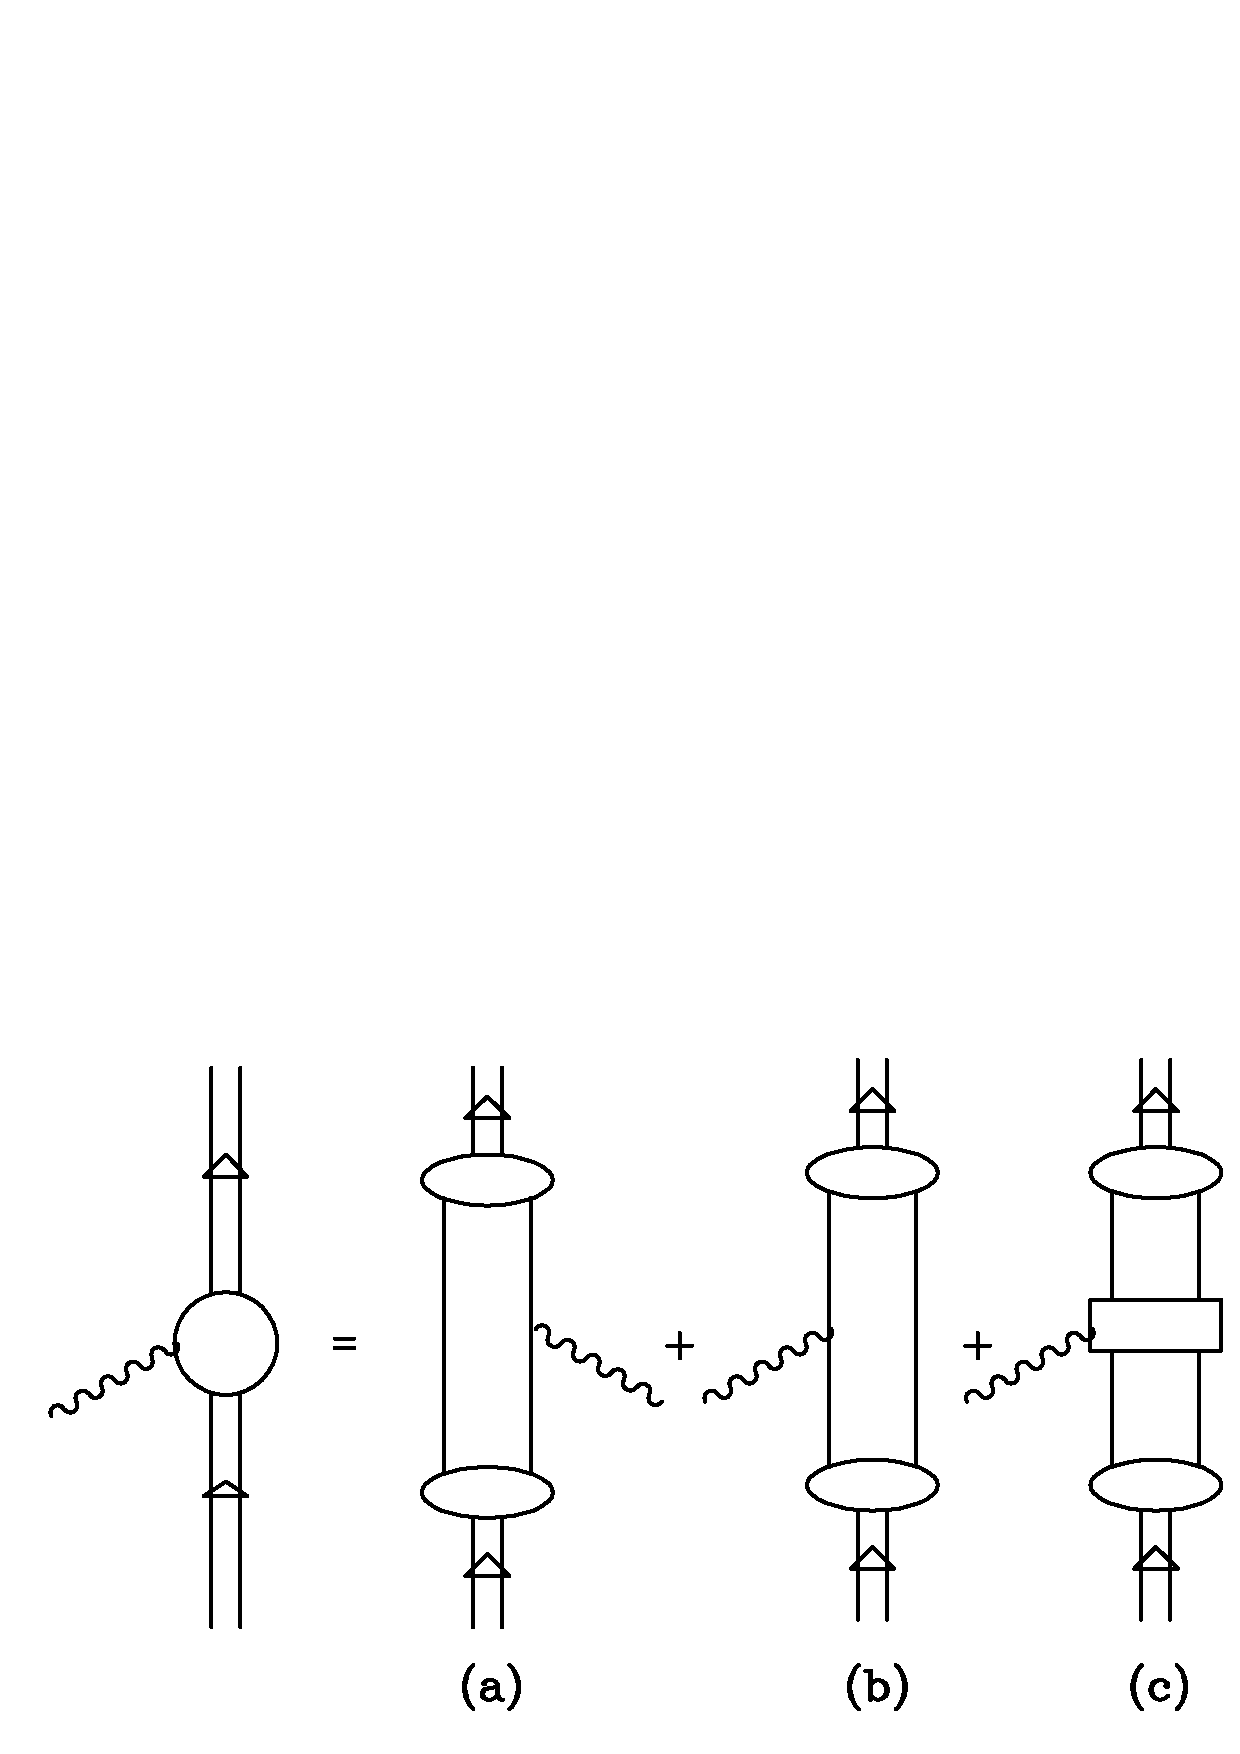
\includegraphics[width=5in]{graphics/new/currntme.pdf}}
\caption{Feynman diagrams representing the Bethe-Salpeter matrix
element for elastic electron scattering form the two-nucleon bound
state} \label{BScurrent}
\end{figure}

\begin{figure}
\centerline{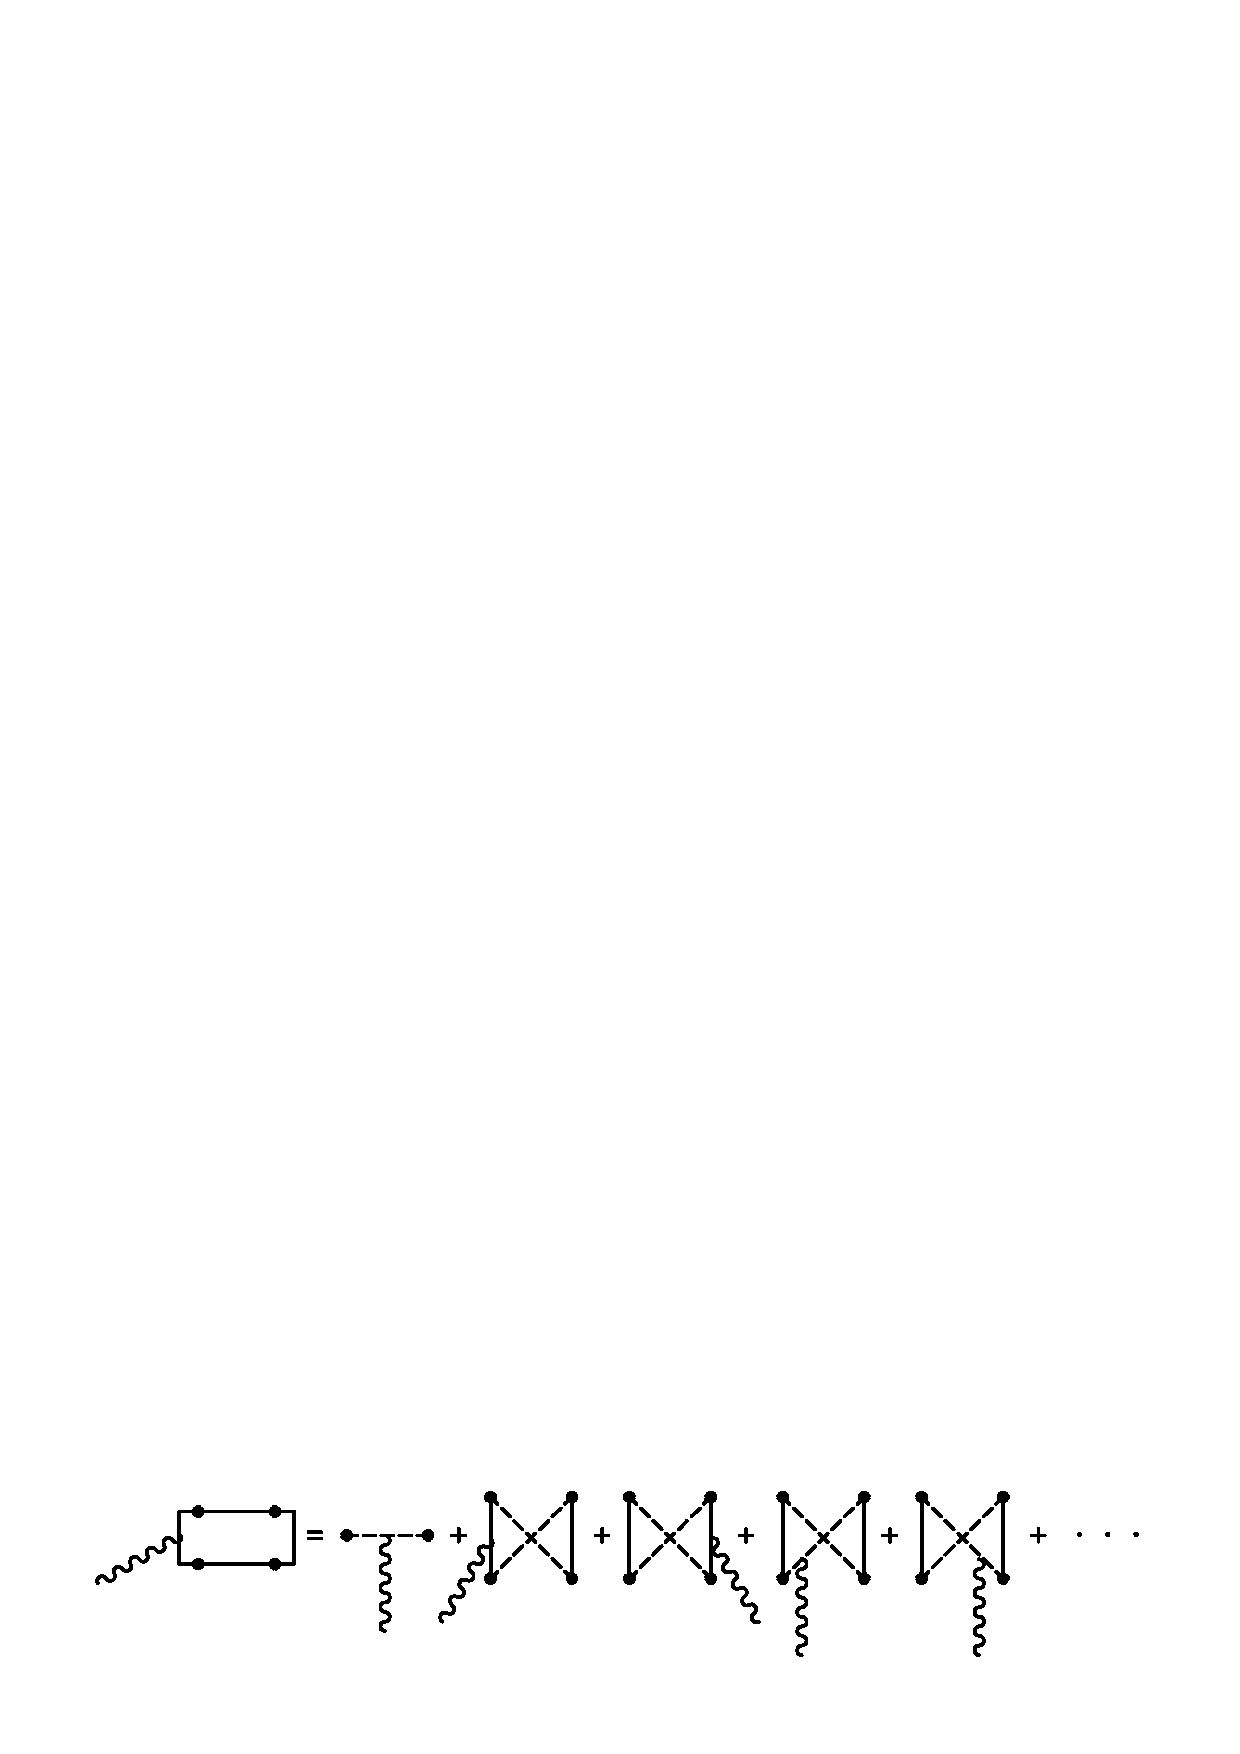
\includegraphics[width=5in]{graphics/new/exchange.pdf}}
\caption{Feynman diagrams representing the two-nucleon irreducible
electromagnetic interaction current.}\label{BSexchange}
\end{figure}

In the simple scalar model, the Feynman rules can be used to represent
the three diagrams in Fig. \ref{BScurrent} as
%
\begin{eqnarray}
{\cal J}^\mu(P',P)&=&-\int\frac{d^4p'}{(2\pi^4)}\int\frac{d^4p}{(2\pi^4)}
\psi^\dagger(p';P') \nonumber \\
&\times&\left\{ i J^{(1)\mu}\left(\frac{P'}{2}+p',\frac{P}{2}+p\right)
{\Delta^{(2)}_F}^{-1}\left(\frac{P'}{2}-p',m\right) \right.  \nonumber \\
& &\times (2\pi)^4
\delta^4\left(\frac{P'}{2}-p'-\frac{P}{2}+p\right) \nonumber \\
& &+i J^{(2)\mu}\left(\frac{P'}{2}-p',\frac{P}{2}-p\right)
{\Delta^{(1)}_F}^{-1}\left(\frac{P'}{2}+p',m\right) \nonumber \\
& &\times (2\pi)^4
\delta^4\left(\frac{P'}{2}+p'-\frac{P}{2}-p\right)
 +J^{(12)\mu}(p',P';p,P)\Biggr\} \psi(p;P)\label{BScurME}
\end{eqnarray}
%
where $J^{(i)\mu}(p'_i,p_i)$ is the single-nucleon current operator for
nucleon $i$ and $J^{(12)\mu}(p',P';p,P)$ is the two-nucleon irreducible
current operator.

The single-nucleon current must satisfy the Ward-Takahashi identity
\cite{WardTakahashi}
%
\begin{equation}
q_\mu J^{(i) \mu}(p',p)=\Delta^{-1}_F(p',m)-\Delta^{-1}_F(p,m).
\label{WardTakahashi1}
\end{equation}
%
Contracting the current matrix element (\ref{BScurME}) with $q_\mu$ and
using the wave equation (\ref{BSwaveEq}), it can be shown that the
two-nucleon current operator must satisfy the identity \cite{GrossandRiska}
%
\begin{eqnarray}
q_\mu J^{(12) \mu}(p',P';p,P)&=&V(p'+\frac{q}{2},p;P)+
V(p'-\frac{q}{2},p;P) \nonumber \\
& &-V(p',p+\frac{q}{2};P')-V(p',p-\frac{q}{2};P')
\label{WardTakahashi2}
\end{eqnarray}

If the model calculations were strictly field theoretical, there would now
be no additional complications, since the usual field theoretical couplings
to the nucleon and meson for the diagrams of Fig. \ref{BSexchange}
would satisfy (\ref{WardTakahashi2}) provided that the kernel and the
two-nucleon current were truncated at the same number of meson exchanges.
The complication comes from the introduction of form factors at the strong
and electromagnetic vertices to account for the finite sizes of the
nucleons and mesons. For example, it is tempting to simply write the
phenomenological electromagnetic one-body current for the nucleon as the
field theoretical bare coupling multiplied by a form factor to give
%
\begin{equation}
J^{(i) \mu}(p',p)=F(Q^2)(p'+p)^\mu
\end{equation}
%
where $Q^2=-q^2=-(p'-p)^2$.
This does not satisfy the Ward-Takahashi identity, however. This problem
has been studied in Ref. \cite{GrossandRiska} for models containing
factorable vertices
such as is defined by (\ref{strongvert}) and (\ref{factorable}). It is
shown there that this problem can be dealt with if the electromagnetic
current is taken to be
%
\begin{equation}
J^{(i) \mu}(p',p)=a(Q^2,p'^2,p^2)\left[ (p'+p)^\mu-\frac{(p'+p)\cdot q}{q^2}
q^\mu\right]+b(p'^2,p^2)(p'+p)^\mu \label{scalaroff}
\end{equation}
%
where
%
\begin{equation}
b(p'^2,p^2)=f_0(p'^2,p^2)=
\left[ \frac{h(p^2)}{h(p'^2)}(p'^2-m^2)
-\frac{h(p'^2)}{h(p^2)}(p^2-m^2)\right] \frac{1}{p'^2-p^2}
\end{equation}
%
and
%
\begin{equation}
a(Q^2,p'^2,p^2)=(F(Q^2)-1)h_0(Q^2,p'^2,p^2)
\end{equation}
%
where $h_0$ is some function subject to the constraint $h_0(Q^2,m^2,m^2)=1$.
The choice $h_0(Q^2,p'^2,p^2)=f_0(p'^2,p^2)$ is used here for simplicity.
A similar procedure must be followed in general for the electromagnetic
current of the meson. For the calculations presented here,  a
single-nucleon form factor of the form
%
\begin{equation}
F(Q^2)=\frac{1}{\left( 1+\frac{Q^2}{0.71 GeV^2}\right)^2}
\end{equation}
is used.


\section{Electromagnetic Current for the Spectator Equation}

Construction of the correct form of the current matrix element for the
truncated quasipotential has not been sufficiently studied for the general
case. However, the correct form of the matrix element for the spectator or
Gross equation has been described in Ref. \cite{GrossandRiska}, and a
description of the
matrix element for the Blankenbecler-Sugar equation is described in a
recent paper by Coester and Riska \cite{CoesterandRiska}. The spectator
equation will be
used for the calculations of the electromagnetic current presented here for
the scalar model and for the realistic deuteron calculation.

\begin{figure}
\centerline{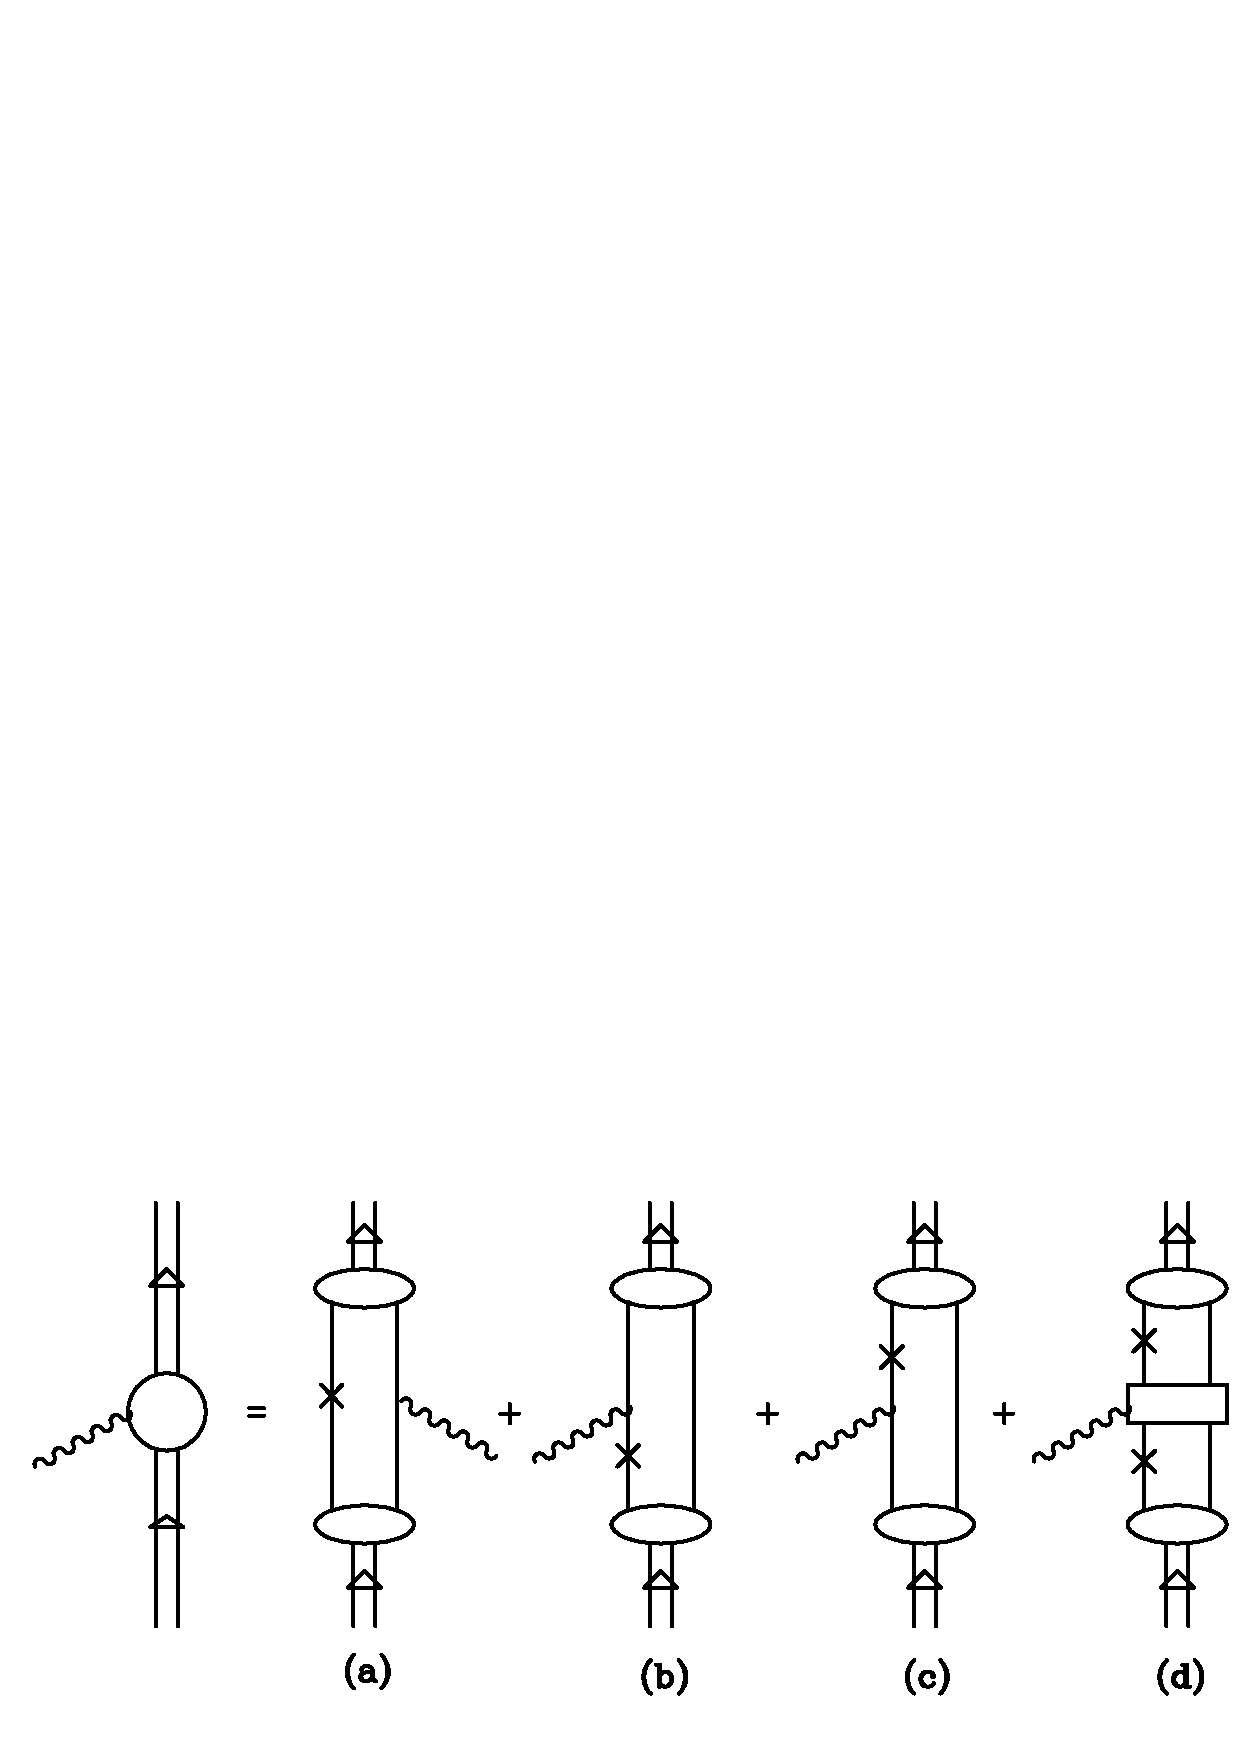
\includegraphics[width=5in]{graphics/new/gcrrntme.pdf}}
\caption{Feynman diagrams representing the elastic current matrix
element for the spectator or Gross equation}\label{Gcurrent}
\end{figure}


The motivation for the construction of the current matrix element for the
spectator equation can be most easily seen by realizing that the choice of
the spectator equation propagator is equivalent to keeping only the
positive energy nucleon pole for particle 1 in all loop integrations. Now,
consider the diagrams for the Bethe-Salpeter current matrix element in
Fig. \ref{BScurrent}. For diagram (\ref{BScurrent}a), particle 1 can be
placed on its positive energy mass shell leading to diagram
(\ref{Gcurrent}a), where the on-shell particle is represented by a cross.
In the case of Fig. \ref{BScurrent}b, particle 1
can be placed on mass shell either before or after the interaction with
the virtual photon leading to the two diagrams (\ref{Gcurrent}b) and
(\ref{Gcurrent}c). Diagram (\ref{BScurrent}c) contains two loops and
particle 1 can be placed on shell in both of them leading to diagram
(\ref{Gcurrent}c). In this last case, the two-nucleon current will be
the same as the Bethe-Salpeter two-nucleon current only at the level of
one meson exchange. Note that while diagrams (\ref{Gcurrent}a) and
(\ref{Gcurrent}d) require only the constrained vertex functions, diagrams
(\ref{Gcurrent}b) and (\ref{Gcurrent}c) require both the constrained and
the unconstrained vertex functions.

Prior to Ref. \cite{GrossandRiska}, it was assumed that the proper form of the current
matrix element was described by diagram (\ref{Gcurrent}a) along with
a symmetric diagram where the photon attaches to particle 1 and particle 2
is placed on mass shell \cite{ACG}. Because of the symmetry of the matrix element, the
contribution of the second diagram is equivalent to
diagram (\ref{Gcurrent}a). Thus this approximation is equivalent to simply
calculating $2\times$diagram (\ref{Gcurrent}a). Since the form of this
approximation looks like a matrix element of a single-nucleon current
between spectator wave functions, it is referred to as the relativistic
impulse approximation (RIA). However, it has been shown that the RIA
does not, in general, conserve the electromagnetic current while the complete
matrix element, described by the diagrams of Fig. \ref{Gcurrent}, does
\cite{GrossandRiska}.

For elastic scattering from the scalar deuteron, Lorentz invariance and
current conservation require that the current matrix element be of the
form
%
\begin{equation}
{\cal J}^\mu(P',P)=G(Q^2)(P'^\mu+P^\mu)
\end{equation}
%
where $G(Q^2)$ is the elastic form factor with $Q^2=-(P'-P)^2$. The form
factor is defined such that $G(0)=1$, since at long wave lengths only the
total charge of the scalar deuteron can be measured. The symptom of the
lack of current conservation in the RIA is manifest as $G_{RIA}(0)\neq 1$.

\begin{figure}
 \centerline{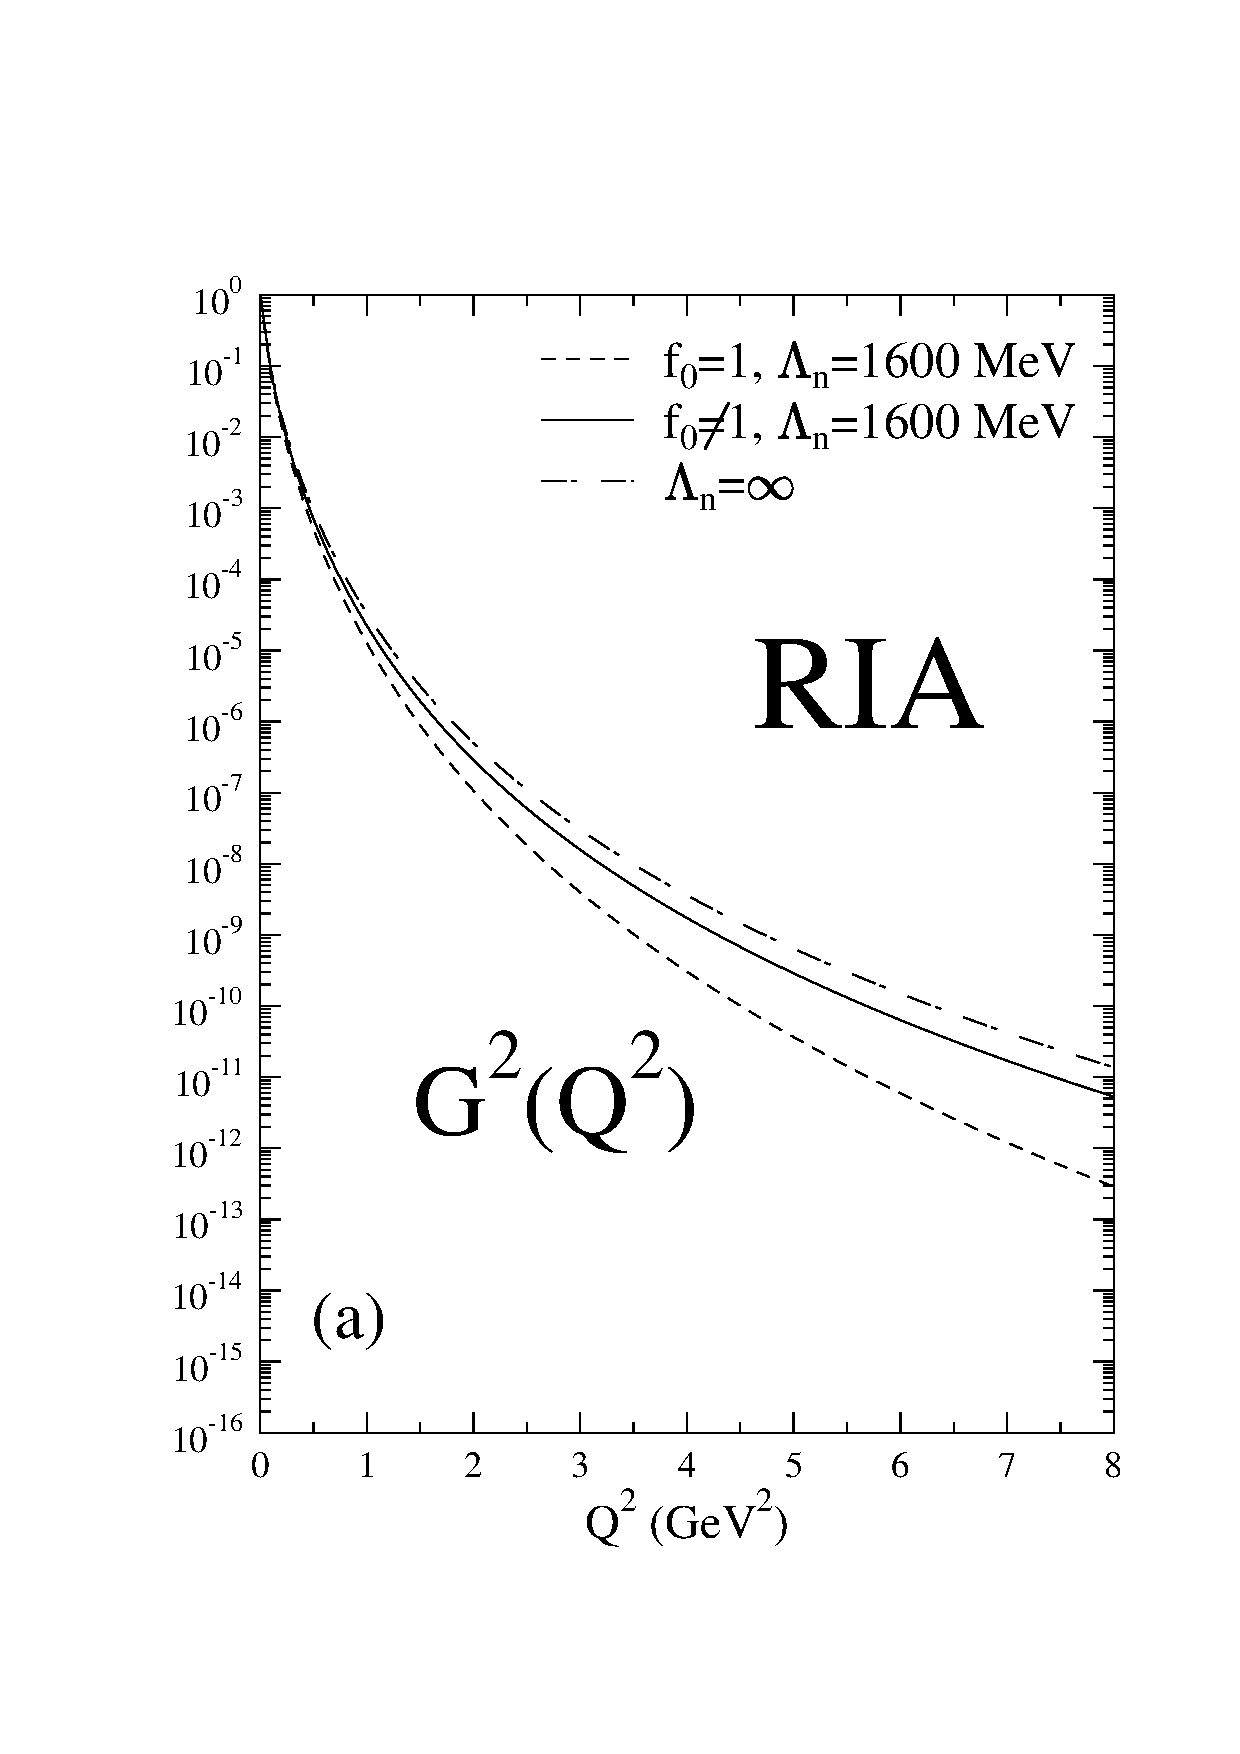
\includegraphics[width=2.75in]{graphics/g_sq_ria.pdf}
             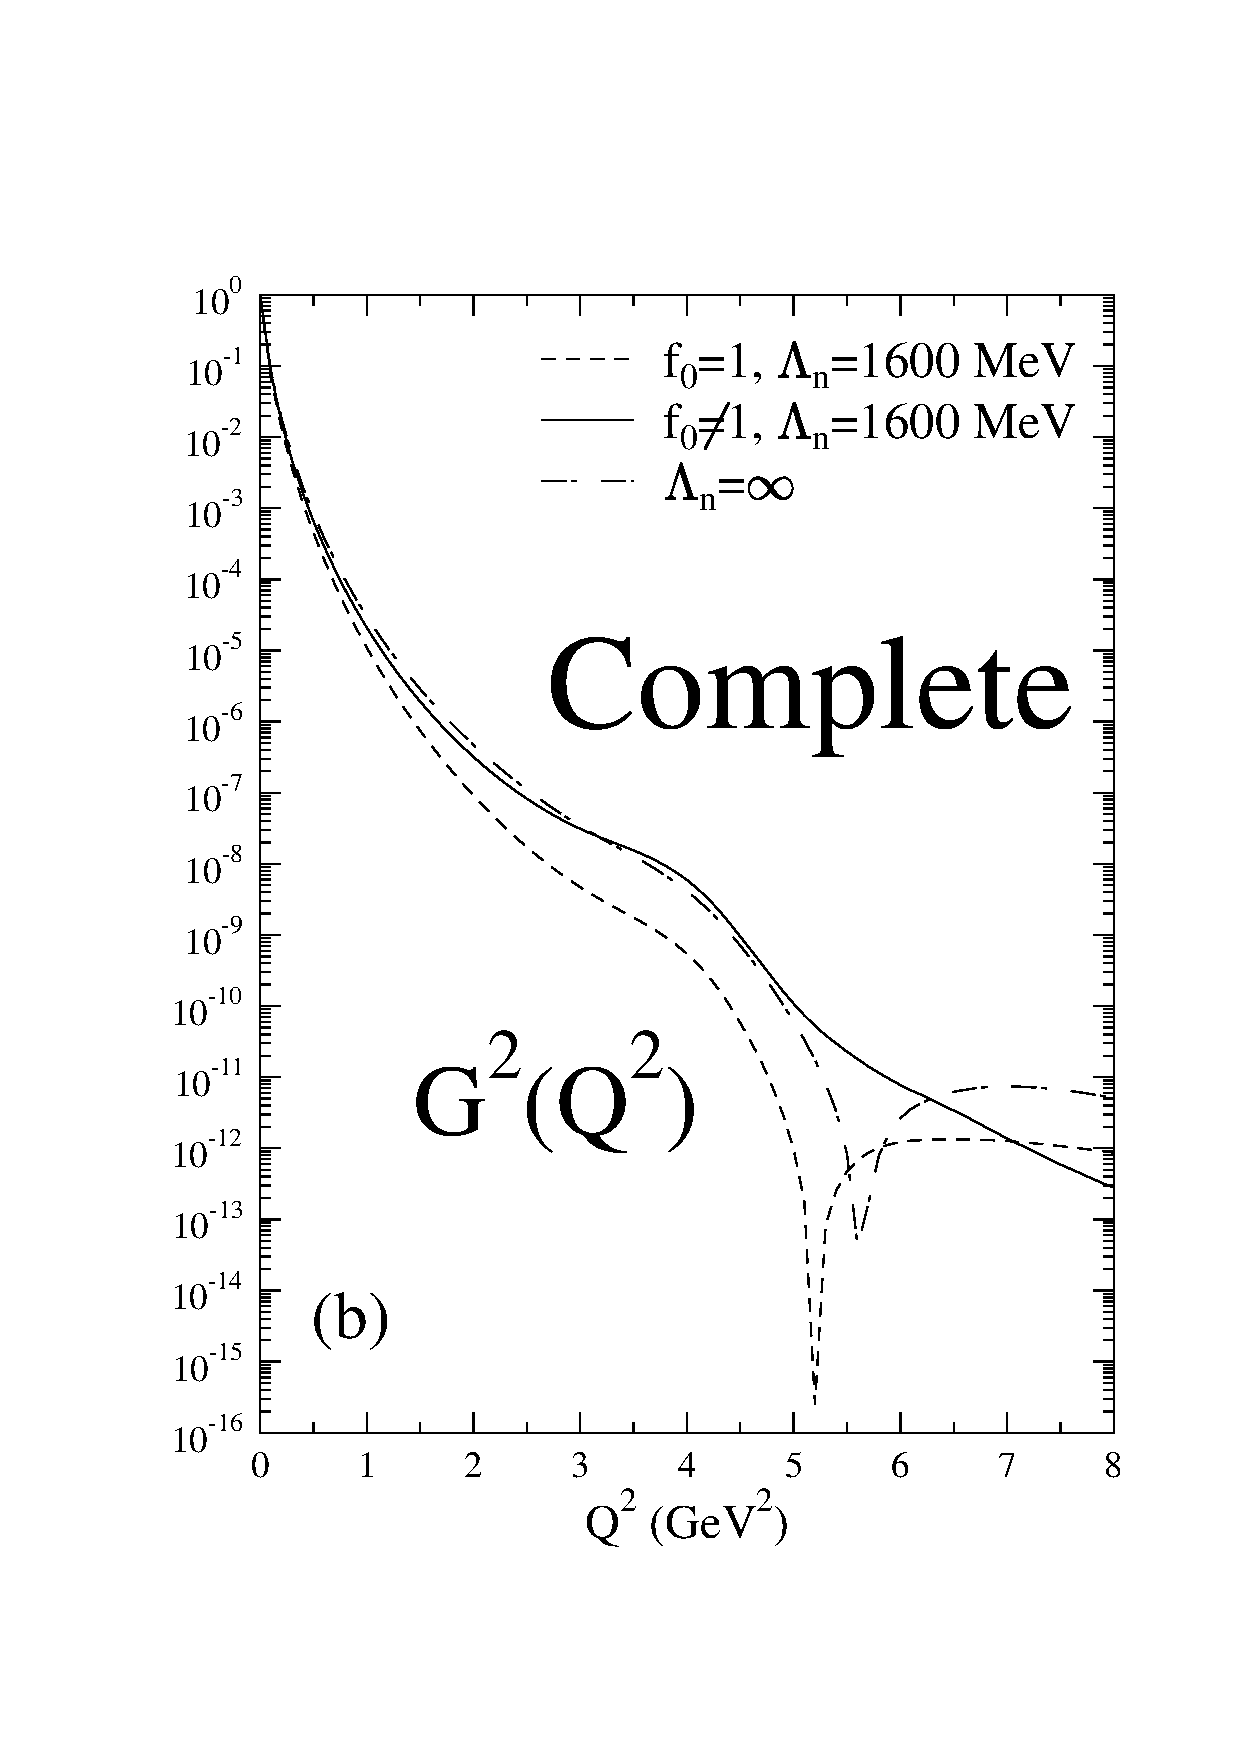
\includegraphics[width=2.75in]{graphics/g_sq_abc.pdf}}
  \caption{The square of the electric form factor of the scalar deuteron.
Figure (a) shows three calculations in the RIA while figure (b)
shows similar calculations for the complete current conserving
matrix element.}\label{scalarff}
\end{figure}

Figure \ref{scalarff} shows the square of the form factor of the scalar
deuteron calculated using the spectator equation. Fig. \ref{scalarff}a
shows three calculations of the RIA, one with $f_0=1$ for
$\Lambda_n=1600~MeV$, one with the single-nucleon current as given in
(\ref{scalaroff}) (labeled as $f_0\neq 1$) for $\Lambda_n=1600~MeV$, and
a the third is calculated with $\Lambda_n=\infty$. Note that the use of
the off-shell current operator (\ref{scalaroff}) results in a substantial
increase in the size of the form factor at large momentum transfers,
bringing it much closer to the result with no nucleon cutoff.
Figure \ref{scalarff}b shows the complete calculation resulting from the
sum of diagrams
(\ref{Gcurrent}a), (\ref{Gcurrent}b) and (\ref{Gcurrent}c), where, in this
case, diagram (\ref{Gcurrent}d) does not contribute since it is assumed
that the meson carries no charge. Three calculations are presented which
correspond to those of Fig. \ref{scalarff}a. The basic trends are as in the
RIA. However, it is clear that calculation of the complete
conserved current can result in a substantial modification of the form
factor at larger momentum transfers from that obtained in the RIA.


\end{document}
